
\documentclass[conference]{IEEEtran}

\usepackage{amsmath}
\usepackage{booktabs}
\usepackage{array}
\usepackage{multirow}
\usepackage{tikz}
\usepackage{xcolor}
\usepackage{listings}
\usepackage{cite}
\usepackage{url}
\usepackage{balance}
\usetikzlibrary{positioning,arrows.meta,calc}

\definecolor{codegray}{gray}{0.96}
\lstset{
  language=C++,
  basicstyle=\ttfamily\scriptsize,
  backgroundcolor=\color{codegray},
  frame=single,
  rulecolor=\color{black!35},
  numbers=left,
  numberstyle=\tiny,
  numbersep=5pt,
  breaklines=true,
  columns=fullflexible,
  keepspaces=true,
  showstringspaces=false,
  tabsize=2,
  captionpos=b
}

\setlength{\textfloatsep}{7pt plus 2pt minus 2pt}
\setlength{\floatsep}{6pt plus 2pt minus 2pt}
\setlength{\intextsep}{6pt plus 2pt minus 2pt}

\title{High-Level Synthesis for Scheduling Pipelined Circuits:\\
A Small List-Based Modulo Scheduler}

\author{
\IEEEauthorblockN{Md Ratul Ahmed Alvi}
\IEEEauthorblockA{
Department of Electrical Engineering\\
Hochschule Hamm-Lippstadt (HSHL)\\
Lippstadt, Germany\\
md-ratul-ahmed.alvi@stud.hshl.de}
}

\begin{document}
\maketitle

\begin{abstract}
High-level synthesis translates behavioral descriptions into register-transfer
level hardware. One important step is scheduling, because the selected start time
of each operation determines resource use, latency, and throughput. For loop-based
designs, modulo scheduling overlaps successive iterations and is mainly described
by the initiation interval (II). This paper presents a small list-based modulo
scheduler written in C++ and explains the resource-constrained and
recurrence-constrained lower bounds on II. Three examples are studied: a 3-tap FIR
filter, an accumulation loop, and a single-multiply delay line. The corrected
experiments show three different situations: a resource-limited schedule, a
recurrence-limited schedule, and a schedule with II equal to one. The examples also
show why operation latency and resource initiation capability must be stated
separately when evaluating a pipelined design.
\end{abstract}

\begin{IEEEkeywords}
high-level synthesis, modulo scheduling, list scheduling, initiation interval,
pipeline, data-flow graph
\end{IEEEkeywords}

\section{Introduction}

Designing a circuit directly in VHDL or Verilog gives the designer detailed
control, but it also requires time and hardware-specific experience. High-level
synthesis (HLS) reduces part of this effort by converting a behavioral description
into an RTL implementation. The main HLS steps include scheduling, allocation, and
binding \cite{demicheli1994}. Scheduling decides when each operation starts and
therefore has a direct effect on performance and resource usage.

Loops are common in signal processing and control applications. If every
iteration is executed completely before the next one starts, the resulting
throughput can be low. Loop pipelining improves throughput by overlapping
successive iterations. The time between the start of two iterations is called the
initiation interval (II). A smaller II normally means a higher steady-state
throughput.

This work studies a small list-based modulo scheduler. The purpose is not to
replace a production HLS tool, but to demonstrate the main scheduling constraints
in a form that can be followed and tested by a student. The paper first introduces
the mathematical model, then describes the scheduler, and finally evaluates three
small examples.

\section{Background}

\subsection{Data-Flow Graph}

A loop body can be represented by a data-flow graph
$G=(V,E)$. Each node $v\in V$ is an operation, and each edge
$e=(u,v,d)$ represents a dependency from operation $u$ to operation $v$.
The value $d$ is the iteration distance. An edge with $d=0$ is inside one
iteration, while $d>0$ is a loop-carried dependency.

For a target initiation interval $II$, a valid modulo schedule must satisfy

\begin{equation}
t(v) \geq t(u)+\lambda(u)-d\cdot II ,
\label{eq:precedence}
\end{equation}

where $t(v)$ is the start time and $\lambda(u)$ is the latency of operation $u$.
Equation~\eqref{eq:precedence} is important because it handles both normal and
loop-carried dependencies.

\subsection{Resource and Recurrence Bounds}

The resource-constrained initiation interval estimates how often the required
operations can be started with the available hardware. If every functional unit
can accept one new operation per cycle, the lower bound is

\begin{equation}
ResII = \max_r \left\lceil \frac{N_r}{M_r} \right\rceil ,
\label{eq:resii}
\end{equation}

where $N_r$ is the number of operations of resource type $r$ in one iteration and
$M_r$ is the number of available units. If a unit is not fully pipelined, its own
initiation interval must also be included in the resource calculation.

A loop-carried cycle with total latency $D$ and iteration distance $L$ gives the
recurrence bound

\begin{equation}
RecII = \left\lceil \frac{D}{L} \right\rceil .
\label{eq:recii}
\end{equation}

The scheduler cannot use an II below

\begin{equation}
II_{\min}=\max(ResII,RecII).
\label{eq:iimin}
\end{equation}

These are lower bounds. A heuristic scheduler may still require a larger II if it
cannot find a feasible placement.

\subsection{Latency and Throughput}

Latency is the time from the start of one iteration until its result is available.
Throughput describes how frequently results are produced after the pipeline has
filled. For one result per iteration,

\begin{equation}
Throughput=\frac{1}{II}.
\label{eq:throughput}
\end{equation}

A pipeline can therefore improve throughput without reducing the latency of one
individual iteration.

\section{List-Based Modulo Scheduler}

The implementation uses a simple iterative approach inspired by modulo scheduling
methods \cite{rau1994,zhang2013}. Operations are first ordered by their ASAP times.
For each target II, the scheduler tries to place every operation at the earliest
cycle that satisfies both dependency and modulo-resource constraints.

\begin{enumerate}
\item Compute $ResII$, $RecII$, and $II_{\min}$.
\item Start with $II=II_{\min}$.
\item Compute an ASAP-based priority order.
\item Place each operation at the earliest valid cycle.
\item Check all dependencies using Eq.~\eqref{eq:precedence}.
\item If the schedule is invalid, increase II and repeat.
\end{enumerate}

The resource table is indexed by $c\bmod II$, because operations from later
iterations repeat in the same modulo slots. Listing~\ref{lst:core} shows the main
idea. The actual program also checks dependencies before accepting a cycle.

\begin{lstlisting}[caption={Simplified greedy placement loop.},
label={lst:core}]
for (int id : order) {
    int c = asap[id];

    while (!dependenciesSatisfied(id, c, II, schedule)
           || resourceUsed(c % II, ops[id].type)
              >= available(ops[id].type)) {
        ++c;
    }

    schedule[id] = c;
    reserve(c % II, ops[id].type);
}
\end{lstlisting}


The program represents each operation with a type, latency, dependency list, and
iteration distance. The minimum information is illustrated in
Listing~\ref{lst:op}.

\begin{lstlisting}[caption={Operation representation used by the scheduler.},
label={lst:op}]
struct Edge {
    int source;
    int distance;
};

struct Op {
    Resource type;
    int latency;
    vector<Edge> deps;
};
\end{lstlisting}

This implementation is deliberately small. Its runtime depends on the number of
operations, the number of tested II values, and how far the cycle search moves
before a free valid slot is found. Therefore, a fixed $O(n\log n)$ claim would be
too strong for the complete implementation. Sorting the priority list costs
$O(n\log n)$, but the repeated feasibility search adds further work.

\section{Experiments}

All examples use fully pipelined functional units: an operation may have a latency
greater than one, but the same unit can accept a new operation every cycle. This
assumption is necessary to interpret Eq.~\eqref{eq:resii} correctly.

\subsection{FIR Filter: Resource-Limited Case}

The first loop implements

\begin{equation}
y[n]=a\,x[n]+b\,x[n-1]+c\,x[n-2].
\end{equation}

It contains three multiplications and two additions. One multiplier and two adders
are available. Multiplier latency is two cycles and adder latency is one cycle.
The graph has no loop-carried dependency.

\begin{figure}[t]
\centering
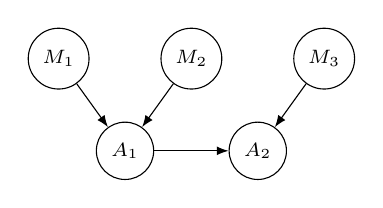
\begin{tikzpicture}[
  op/.style={draw,circle,minimum size=7mm,font=\scriptsize},
  arr/.style={-{Latex[length=1.5mm]},thin},
  node distance=8mm and 9mm
]
\node[op] (m1) {$M_1$};
\node[op,right=of m1] (m2) {$M_2$};
\node[op,right=of m2] (m3) {$M_3$};
\node[op,below=of $(m1)!0.5!(m2)$] (a1) {$A_1$};
\node[op,below=of $(m2)!0.5!(m3)$] (a2) {$A_2$};
\draw[arr] (m1) -- (a1);
\draw[arr] (m2) -- (a1);
\draw[arr] (a1) -- (a2);
\draw[arr] (m3) -- (a2);
\end{tikzpicture}
\caption{Data-flow graph of the 3-tap FIR loop.}
\label{fig:fir}
\end{figure}

The resource bound is

\begin{equation}
ResII=\left\lceil\frac{3}{1}\right\rceil=3,
\qquad RecII=0.
\end{equation}

The scheduler finds $II=3$, which reaches the lower bound. Table~\ref{tab:fir}
shows one modulo schedule. The three multiplier starts occupy the three modulo
slots, while the two additions use separate adder resources.

\begin{table}[t]
\centering
\caption{FIR schedule for one iteration, $II=3$.}
\label{tab:fir}
\begin{tabular}{@{}ccc@{}}
\toprule
Operation & Start cycle & Resource\\
\midrule
$M_1$ & 0 & Multiplier\\
$M_2$ & 1 & Multiplier\\
$M_3$ & 2 & Multiplier\\
$A_1$ & 3 & Adder\\
$A_2$ & 4 & Adder\\
\bottomrule
\end{tabular}
\end{table}

The result latency is five cycles, while a new iteration starts every three
cycles. The steady-state throughput is therefore $1/3$ result per cycle.

\subsection{Accumulation: Recurrence-Limited Case}

The second loop is

\begin{equation}
sum \mathrel{+}= x[i]\cdot coeff .
\end{equation}

One multiplier and one adder are available. Both units are fully pipelined.
Multiplier latency is two cycles. To create a clear recurrence-limited example,
the accumulator addition is modeled with latency two cycles. Its result is used by
the next iteration, giving a recurrence with $D=2$ and $L=1$.

\begin{figure}[t]
\centering
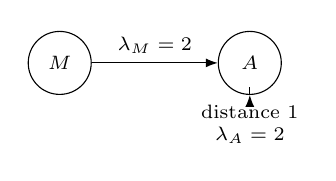
\begin{tikzpicture}[
  op/.style={draw,circle,minimum size=8mm,font=\scriptsize},
  arr/.style={-{Latex[length=1.5mm]},thin},
  rec/.style={-{Latex[length=1.5mm]},thin,dashed},
  node distance=16mm
]
\node[op] (m) {$M$};
\node[op,right=of m] (a) {$A$};
\draw[arr] (m) -- node[above,font=\scriptsize] {$\lambda_M=2$} (a);
\draw[rec] (a.south) to[out=-100,in=-80,looseness=2.2]
node[below,font=\scriptsize,align=center]{distance $1$\\$\lambda_A=2$} (a.south);
\end{tikzpicture}
\caption{Accumulation loop with a loop-carried recurrence.}
\label{fig:acc}
\end{figure}

The bounds are

\begin{equation}
ResII=1,\qquad
RecII=\left\lceil\frac{2}{1}\right\rceil=2.
\end{equation}

The scheduler therefore starts at $II_{\min}=2$ and finds a feasible schedule.
Table~\ref{tab:acc} shows the repeated start pattern.

\begin{table}[t]
\centering
\caption{Accumulation schedule, $II=2$.}
\label{tab:acc}
\begin{tabular}{@{}cccccc@{}}
\toprule
Iteration & $M$ start & $A$ start & Result\\
\midrule
0 & 0 & 2 & 4\\
1 & 2 & 4 & 6\\
2 & 4 & 6 & 8\\
3 & 6 & 8 & 10\\
\bottomrule
\end{tabular}
\end{table}

This is a genuine recurrence-limited result. Adding more multipliers or adders
does not reduce II below two unless the recurrence is restructured or its latency
is reduced.

\subsection{Delay Line: II Equal to One}

The third loop computes

\begin{equation}
y[n]=x[n]\cdot coeff .
\end{equation}

It contains one multiplication per iteration, two multipliers are available, and
there is no loop-carried dependency. Thus,

\begin{equation}
ResII=1,\qquad RecII=0,\qquad II=1.
\end{equation}

The multiplier latency remains two cycles, but a new iteration begins every cycle.
After the pipeline is filled, one result is produced per cycle.

\begin{table}[t]
\centering
\caption{Delay-line schedule, $II=1$.}
\label{tab:delay}
\begin{tabular}{@{}cccc@{}}
\toprule
Iteration & Multiply start & Result cycle\\
\midrule
0 & 0 & 2\\
1 & 1 & 3\\
2 & 2 & 4\\
3 & 3 & 5\\
4 & 4 & 6\\
\bottomrule
\end{tabular}
\end{table}

\subsection{Summary}

Table~\ref{tab:summary} compares the three cases. The results match the intended
lower bound in each example.


\begin{table}[t]
\centering
\caption{Summary of corrected experiments.}
\label{tab:summary}
\begin{tabular}{@{}lccc@{}}
\toprule
Example & $ResII$ & $RecII$ & II\\
\midrule
3-tap FIR & 3 & 0 & 3\\
Accumulation & 1 & 2 & 2\\
Delay line & 1 & 0 & 1\\
\bottomrule
\end{tabular}
\end{table}




\subsection{Validation Method}

Each experiment was checked in three steps. First, the analytical lower bounds
were calculated using Eqs.~\eqref{eq:resii}--\eqref{eq:iimin}. Second, the C++
scheduler generated start times for all operations. Third, an independent
validation routine checked every dependency and every modulo-resource slot.

For each edge $(u,v,d)$, the validator evaluates Eq.~\eqref{eq:precedence}. For
each resource type, it also counts the operation starts mapped to every
$c\bmod II$ slot. A schedule is accepted only when all dependency inequalities
hold and no slot uses more units than are available. These checks are small, but
they prevent the scheduler from reporting a result that only appears feasible.

The experiments were deliberately chosen so that one expected limit was clear in
each case. This made it possible to compare the observed II with a known
analytical expectation instead of reporting the program output without a
reference value.

\section{Hardware/Software Co-Design View}

The experiment can also be understood as a small hardware/software co-design
workflow. The scheduling algorithm runs as software and receives a behavioral
model, operation latencies, dependency information, and resource limits. Its
output is a cycle-level schedule. That schedule then guides the hardware
architecture by showing when multipliers and adders are required and which
operations may share the same unit.

\begin{figure}[t]
\centering
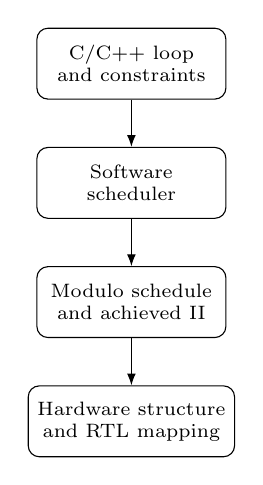
\begin{tikzpicture}[
  block/.style={draw,rounded corners,minimum width=24mm,minimum height=9mm,
  align=center,font=\scriptsize},
  arr/.style={-{Latex[length=1.5mm]},thin},
  node distance=6mm
]
\node[block] (input) {C/C++ loop\\and constraints};
\node[block,below=of input] (sched) {Software\\scheduler};
\node[block,below=of sched] (result) {Modulo schedule\\and achieved II};
\node[block,below=of result] (rtl) {Hardware structure\\and RTL mapping};
\draw[arr] (input) -- (sched);
\draw[arr] (sched) -- (result);
\draw[arr] (result) -- (rtl);
\end{tikzpicture}
\caption{Simplified hardware/software co-design flow used in this work.}
\label{fig:codesign}
\end{figure}

The software side performs design-space reasoning: it tests the lower bounds,
searches for valid start times, and reports whether the current resource budget is
sufficient. The hardware side is represented by the selected number of functional
units and their pipeline behavior. For example, the FIR result shows that one
multiplier forces three multiplication start slots per iteration. This information
can be used to decide whether the extra area of a second multiplier is justified by
a lower II.

The separation is useful because hardware changes can be evaluated first at the
scheduling level. However, the schedule is still only a model. A complete flow
would also generate RTL, synthesize it for an FPGA, and compare the predicted II
with simulation and timing reports.

\section{Discussion}

The examples show why the dominant bound must be identified before changing the
hardware. In the FIR filter, the resource bound dominates. Adding a second
multiplier could lower $ResII$, although a new schedule would still be required.
In the accumulation loop, the recurrence dominates. Additional units alone do not
change the two-cycle feedback path. In the delay line, neither bound is greater
than one.

The corrected accumulation example also shows an important modeling lesson.
An ordinary dependency from a multiplication to an addition inside the same
iteration does not by itself create $RecII$. A recurrence bound requires a
loop-carried dependency. The latency around that loop-carried cycle and its
iteration distance determine Eq.~\eqref{eq:recii}.

The implementation remains a teaching model. Production modulo schedulers handle
memory dependencies, control flow, chaining, operator-specific initiation
intervals, and schedule-length optimization. Exact formulations can prove optimal
IIs for many practical loops, but they are more complex than the list-based
approach used here \cite{oppermann2019}. Heuristic and SDC-based approaches offer
other trade-offs between scheduling quality and runtime \cite{zhang2013}.

\balance
\section{Conclusion}

This paper presented a small list-based modulo scheduler for pipelined loops in
HLS. The scheduler starts from the maximum of the resource and recurrence bounds
and increases II only when a feasible schedule cannot be found.

Three corrected examples demonstrated different limits. The FIR filter reached
$II=3$ because one multiplier had to start three multiplications per iteration.
The accumulation loop reached $II=2$ because of a two-cycle loop-carried
recurrence. The delay line reached $II=1$ because neither resources nor
dependencies required a larger interval. The main result is that operation
latency, functional-unit initiation capability, and loop-carried dependence must
be modeled separately. Without this distinction, an observed II can easily be
attributed to the wrong cause.


\begin{thebibliography}{00}

\bibitem{demicheli1994}
G. De Micheli, \emph{Synthesis and Optimization of Digital Circuits}.
New York, NY, USA: McGraw-Hill, 1994.

\bibitem{rau1994}
B. R. Rau, ``Iterative modulo scheduling: An algorithm for software-pipelining
loops,'' in \emph{Proc. 27th Annu. Int. Symp. Microarchitecture}, 1994,
pp. 63--74.

\bibitem{zhang2013}
Z. Zhang and B. Liu, ``SDC-based modulo scheduling for pipeline synthesis,''
in \emph{Proc. IEEE/ACM Int. Conf. Computer-Aided Design}, 2013,
pp. 211--218.

\bibitem{oppermann2019}
J. Oppermann, M. Reuter-Oppermann, L. Sommer, A. Koch, and O. Sinnen,
``Exact and practical modulo scheduling for high-level synthesis,''
\emph{ACM Trans. Reconfigurable Technol. Syst.}, vol. 12, no. 2,
pp. 1--26, 2019.

\end{thebibliography}


\end{document}
